\documentclass[11pt]{article}
\usepackage[a4paper,margin=1in]{geometry}
\usepackage{fontspec}
\setmainfont{TeX Gyre Termes}
\usepackage{booktabs}
\usepackage{tabularx}
\usepackage{longtable}
\usepackage{array}
\usepackage{ragged2e}
\usepackage{hyperref}
\usepackage{xcolor}
\usepackage{tikz}
\usetikzlibrary{positioning}
\usepackage{caption}
\usepackage{float}

\hypersetup{colorlinks=true,linkcolor=blue,citecolor=blue,urlcolor=blue}
\newcolumntype{Y}{>{\RaggedRight\arraybackslash}X}

\title{A Systematic Literature Review of Embedding Models for Vietnamese Text Retrieval with a Focus on Vietnamese Historical Documents}
\author{Undergraduate Research Draft}
\date{June 2026}

\begin{document}
\maketitle

\begin{abstract}
This systematic literature review examines embedding models for Vietnamese text retrieval, with a focus on Vietnamese historical documents. The study synthesizes existing evidence only: it does not introduce a new benchmark, run experiments, or claim new empirical results. Sources were searched across ACL Anthology, arXiv, TACL, OpenReview, ScienceDirect, official model cards, and benchmark pages. The strongest evidence is for general Vietnamese retrieval, Vietnamese embedding benchmarks, and Vietnamese legal retrieval, while evidence for Vietnamese historical document retrieval remains indirect. No direct benchmark evidence was found for Vietnamese historical document retrieval. Therefore, Hybrid BM25 + BGE-M3 and multilingual E5 should be treated as practical first candidates, not proven best models. Historical retrieval still requires pilot validation on representative documents. Because historical PDFs may contain scans, old fonts, footnotes, names, dates, and OCR errors, the review recommends page-aware extraction, OCR only when needed, hybrid sparse+dense retrieval, and citation-preserving retrieval as a conservative first setup.
\end{abstract}

\section{Introduction}
Vietnamese text retrieval is increasingly important for search, question answering, and retrieval-augmented generation. Recent Vietnamese benchmarks such as VN-MTEB \cite{pham-etal-2026-vn}, a multi-domain Vietnamese IR study \cite{nguyen-quan-2026-works}, and Vietnamese Context Search \cite{nguyen-etal-2024-advancing} make it possible to discuss embedding models with more evidence than before. Legal retrieval studies also provide useful specialized-domain evidence \cite{khang-etal-2024-vietnamese-legal,nguyen-etal-2025-improving,ba-etal-2024-vietnamese-legal-ir}.

Embedding selection matters because dense models, sparse lexical methods, hybrid retrieval, and reranking behave differently across datasets and domains. Historical documents add further difficulty: they may contain scanned pages, old fonts, page headers, footnotes, names, dates, event chains, and OCR errors. This review therefore avoids claiming a single best model. Its central conclusion is that existing literature supports practical candidates, especially Hybrid BM25 + BGE-M3 and multilingual E5, but not an absolute best model for Vietnamese historical document retrieval.

\section{Research Questions}
\begin{enumerate}
\item RQ1: What embedding models and retrieval methods have been studied for Vietnamese text retrieval?
\item RQ2: What evidence exists for their suitability to Vietnamese historical documents?
\item RQ3: What practical retrieval setup should be considered when direct history benchmarks are unavailable?
\end{enumerate}

\section{Methodology}
\subsection{Search Strategy and Criteria}
The review searched academic and official sources including ACL Anthology, arXiv, TACL, OpenReview, ScienceDirect, Hugging Face model cards, official benchmark pages, and official documentation. Search terms included Vietnamese dense retrieval, Vietnamese legal retrieval embedding, VN-MTEB, multilingual E5 Vietnamese retrieval, BGE-M3 Vietnamese retrieval, PhoBERT sentence embedding retrieval, Vietnamese historical document retrieval, and Vietnamese OCR historical documents retrieval.

\begin{table}[H]
\centering
\caption{Search Strategy and Databases}
\label{tab:search}
\small
\begin{tabularx}{\textwidth}{p{0.24\textwidth}Y}
\toprule
Source group & Examples \\
\midrule
Academic sources & ACL Anthology, arXiv, TACL, OpenReview, ScienceDirect. \\
Benchmarks and datasets & VN-MTEB, MTEB, BEIR, MIRACL, mMARCO, Vietnamese retrieval datasets. \\
Model documentation & BGE-M3, multilingual E5, GTE multilingual, Hugging Face model cards. \\
Gap-driven searches & Vietnamese historical retrieval, Vietnamese OCR historical documents, Vietnamese history RAG. \\
\bottomrule
\end{tabularx}
\end{table}

\begin{table}[H]
\centering
\caption{Inclusion and Exclusion Criteria}
\label{tab:criteria}
\small
\begin{tabularx}{\textwidth}{p{0.48\textwidth}p{0.48\textwidth}}
\toprule
Included & Excluded \\
\midrule
Peer-reviewed papers, arXiv reports, benchmark papers, technical reports, official model cards, and official dataset pages. & Blog-only, unverifiable, broken, unrelated, generation-only, or search-result-only sources. \\
Sources about Vietnamese retrieval, multilingual retrieval including Vietnamese, Vietnamese-specific models, retrieval benchmarks, OCR, or PDF processing. & English-only retrieval with no Vietnamese or multilingual relevance, or sources with no usable metadata. \\
\bottomrule
\end{tabularx}
\end{table}

\subsection{Screening and Evidence Strength}
Records were deduplicated by DOI, arXiv ID, ACL Anthology ID, and normalized title. Table~\ref{tab:prisma} reports approximate PRISMA-style counts based on available search results and opened official pages.

\begin{table}[H]
\centering
\caption{PRISMA Flow Summary}
\label{tab:prisma}
\small
\begin{tabularx}{\textwidth}{p{0.52\textwidth}p{0.18\textwidth}Y}
\toprule
Stage & Count & Notes \\
\midrule
Records identified & 73 & Approximate based on available search results. \\
Duplicates removed & 18 & DOI, arXiv ID, ACL ID, and title deduplication. \\
Title/abstract screened & 55 & Retrieval, embedding, benchmark, OCR, and Vietnamese relevance screened. \\
Excluded at title/abstract & 31 & Unrelated, generation-only, unsupported, or non-Vietnamese-only. \\
Full text or official page assessed & 24 & Open PDFs/pages inspected where available. \\
Excluded after full-text/page review & 6 & Insufficient retrieval relevance or verification. \\
Included in synthesis & 18 & Core and supporting sources. \\
\bottomrule
\end{tabularx}
\end{table}

\begin{figure}[H]
\centering
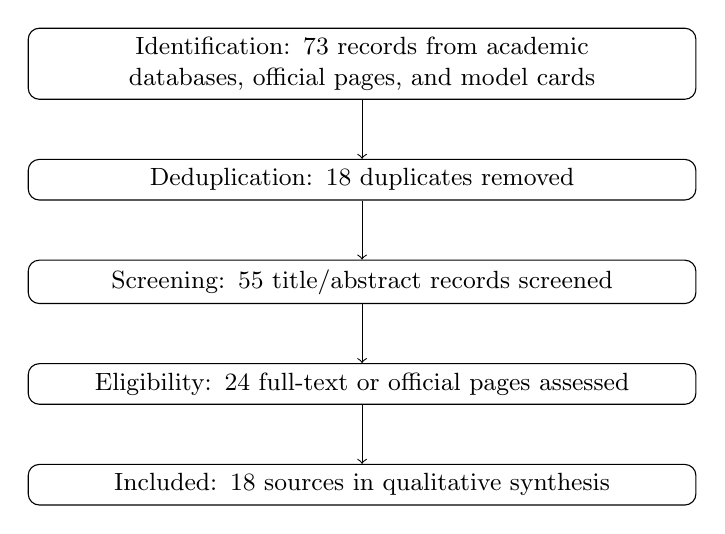
\begin{tikzpicture}[node distance=0.75cm, every node/.style={draw, rounded corners, align=center, font=\small, text width=0.68\textwidth}]
\node (id) {Identification: 73 records from academic databases, official pages, and model cards};
\node (dedup) [below=of id] {Deduplication: 18 duplicates removed};
\node (screen) [below=of dedup] {Screening: 55 title/abstract records screened};
\node (elig) [below=of screen] {Eligibility: 24 full-text or official pages assessed};
\node (inc) [below=of elig] {Included: 18 sources in qualitative synthesis};
\draw[->] (id) -- (dedup);
\draw[->] (dedup) -- (screen);
\draw[->] (screen) -- (elig);
\draw[->] (elig) -- (inc);
\end{tikzpicture}
\caption{PRISMA-style flow diagram. Counts are approximate based on available search results.}
\label{fig:prisma}
\end{figure}

Evidence strength was classified as strong when a source reported direct Vietnamese retrieval evaluation with clear datasets and metrics; moderate when evidence was multilingual or Vietnamese-related but outside the historical domain; weak when evidence came mainly from model cards or indirect related work; and insufficient when no reliable direct evidence was found.

\section{PRISMA Screening Results}
The search found direct evidence for general Vietnamese retrieval, Vietnamese embedding benchmarks, and legal retrieval. It found OCR-related work relevant to historical materials \cite{nguyen-thiet-2025-sinovietnamese-ocr,zhang-etal-2024-ocr-hinders-rag}, but no verified benchmark comparing embedding models on Vietnamese historical document retrieval. Detailed citation audit and browser verification were maintained in the companion deliverables.

\section{Results}
\subsection{Overview of Selected Studies}
\begin{longtable}{p{0.21\textwidth}p{0.28\textwidth}p{0.43\textwidth}}
\caption{Core Studies Included in the Review}
\label{tab:core-studies}\\
\toprule
Citation & Focus & Main relevance \\
\midrule
\endfirsthead
\toprule
Citation & Focus & Main relevance \\
\midrule
\endhead
\cite{pham-etal-2026-vn} & VN-MTEB & Vietnamese embedding benchmark across retrieval and other embedding tasks. \\
\cite{nguyen-quan-2026-works} & Multi-domain Vietnamese IR & Direct Vietnamese retrieval evidence across domains. \\
\cite{nguyen-etal-2024-advancing} & Vietnamese Context Search & Vietnamese retrieval and reranking benchmark. \\
\cite{khang-etal-2024-vietnamese-legal,nguyen-etal-2025-improving,ba-etal-2024-vietnamese-legal-ir} & Vietnamese legal retrieval & Domain-specific evidence for sparse, dense, hybrid, and cross-lingual retrieval. \\
\cite{chen-etal-2024-m3} & BGE-M3 & Multilingual dense, sparse, and multi-vector embedding evidence. \\
\cite{wang-etal-2024-me5} & multilingual E5 & Multilingual embedding training and retrieval evidence. \\
\cite{nguyen-tuan-nguyen-2020-phobert,reimers-gurevych-2019-sentence} & PhoBERT/SBERT & Vietnamese backbone and bi-encoder method evidence. \\
\cite{thakur-etal-2021-beir,muennighoff-etal-2023-mteb} & BEIR/MTEB & General benchmark context and baseline caution. \\
\cite{zhang-etal-2023-miracl,bonifacio-etal-2021-mmarco} & Multilingual retrieval resources & Background for multilingual retrieval and passage ranking. \\
\cite{zhang-etal-2024-ocr-hinders-rag} & OCR and RAG & Evidence that OCR quality can affect retrieval-augmented systems. \\
\bottomrule
\end{longtable}

\subsection{Embedding Models and Retrieval Evidence}
BGE-M3 supports dense, sparse, and multi-vector retrieval, more than 100 working languages, and long sequences up to 8192 tokens \cite{chen-etal-2024-m3}. These properties make it a plausible hybrid candidate, but not a proven historical retrieval model. multilingual E5 is trained with multilingual contrastive and supervised retrieval data \cite{wang-etal-2024-me5}. GTE multilingual is included as a secondary candidate because its official model card reports long context, dense and sparse support, and more than 70 languages \cite{alibaba-nlp-2026-gte-multilingual-base}. LaBSE is a useful older cross-lingual baseline \cite{feng-etal-2022-language}.

Vietnamese-specific evidence is mixed. PhoBERT is a strong Vietnamese language-model backbone, although its original paper is not a retrieval evaluation \cite{nguyen-tuan-nguyen-2020-phobert}. VN-MTEB includes Vietnamese-adapted models such as Vietnamese-Embedding, halong-embedding, vietnamese-bi-encoder, and SimCSE PhoBERT variants \cite{pham-etal-2026-vn}. Legal retrieval papers show the value of sparse, dense, and hybrid approaches in a specialized Vietnamese domain \cite{khang-etal-2024-vietnamese-legal,ba-etal-2024-vietnamese-legal-ir}.

\begin{table}[H]
\centering
\caption{Model Evidence Table}
\label{tab:model-evidence}
\small
\begin{tabularx}{\textwidth}{p{0.18\textwidth}p{0.18\textwidth}Y p{0.22\textwidth}}
\toprule
Model & Type & Evidence & Recommended use \\
\midrule
BGE-M3 & Multilingual & VN-MTEB inclusion; dense/sparse/multi-vector model paper. & First hybrid candidate. \\
multilingual E5 & Multilingual & VN-MTEB inclusion; multilingual retrieval technical report. & Strong baseline candidate. \\
gte-multilingual-base & Multilingual & VN-MTEB inclusion; official model card. & Secondary candidate. \\
PhoBERT/SBERT variants & Vietnamese-specific & PhoBERT backbone; SBERT method; VN-MTEB variants. & Fine-tuning candidate. \\
BM25 & Lexical baseline & BEIR and Vietnamese studies support lexical baselines. & Required baseline. \\
Hybrid BM25+dense & Hybrid system & Supported by BEIR lessons, BGE-M3 functionality, and legal retrieval evidence. & Recommended first pipeline. \\
\bottomrule
\end{tabularx}
\end{table}

\subsection{Datasets, Domains, and Metrics}
VN-MTEB includes Vietnamese retrieval datasets adapted from BEIR/MTEB families, including ArguAna-VN, SciFact-VN, FiQA2018-VN, MSMARCO-VN, NFCorpus-VN, NQ-VN, HotpotQA-VN, and TRECCOVID-VN \cite{pham-etal-2026-vn}. MIRACL and mMARCO provide multilingual background evidence, while BEIR and MTEB frame common metrics such as nDCG, MRR, recall, MAP, and task-specific scores \cite{zhang-etal-2023-miracl,bonifacio-etal-2021-mmarco,thakur-etal-2021-beir,muennighoff-etal-2023-mteb}.

\begin{table}[H]
\centering
\caption{Dataset, Domain, and Metric Table}
\label{tab:datasets}
\small
\begin{tabularx}{\textwidth}{p{0.26\textwidth}p{0.25\textwidth}Y}
\toprule
Dataset or benchmark & Domain & Relevance \\
\midrule
VN-MTEB & General, QA, medical, finance, science, web & Direct Vietnamese embedding evaluation. \\
ViRE & Education, legal, healthcare, support, reviews, open-domain & Direct multi-domain Vietnamese IR evidence. \\
VCS & Vietnamese retrieval and reranking & Vietnamese benchmark evidence. \\
Vietnamese legal datasets & Legal QA and legal article retrieval & Strong domain-specific evidence, but not historical. \\
MTEB/BEIR/MIRACL & General and multilingual retrieval & Background metrics and baseline context. \\
\bottomrule
\end{tabularx}
\end{table}

\subsection{Evidence for Vietnamese Historical Document Retrieval}
No direct benchmark evidence was found for Vietnamese historical document retrieval. Existing recommendations are therefore based on indirect Vietnamese, multilingual, and domain-specific evidence. Historical materials add scanned pages, old fonts, mixed orthography, footnotes, page headers, named entities, dates, and OCR noise. OCR-related studies show that extraction quality can become a retrieval and RAG bottleneck \cite{zhang-etal-2024-ocr-hinders-rag,nguyen-thiet-2025-sinovietnamese-ocr}.

\begin{table}[H]
\centering
\caption{Evidence Strength by Domain}
\label{tab:evidence-domain}
\small
\begin{tabularx}{\textwidth}{p{0.24\textwidth}p{0.18\textwidth}Y}
\toprule
Domain & Evidence strength & Rationale \\
\midrule
General Vietnamese retrieval & Strong & Multi-domain Vietnamese IR, VN-MTEB, and VCS provide direct retrieval evidence. \\
Vietnamese legal retrieval & Strong & Multiple legal retrieval papers and datasets are available. \\
Vietnamese medical retrieval & Moderate & VN-MTEB includes medical-style retrieval datasets, but direct medical retrieval evidence is narrower. \\
Multilingual retrieval including Vietnamese & Moderate & MIRACL, mMARCO, E5, BGE-M3, and VN-MTEB provide indirect evidence. \\
Vietnamese historical retrieval & Insufficient & No verified direct embedding benchmark was found. \\
OCR for historical Vietnamese documents & Weak to moderate & OCR and Han-Nom evidence exists, but not retrieval benchmarking. \\
\bottomrule
\end{tabularx}
\end{table}

\section{Discussion}
The evidence supports a candidate-first rather than winner-first conclusion. VN-MTEB, Vietnamese multi-domain IR, legal retrieval, and general benchmarks use different datasets, domains, metrics, and model settings \cite{pham-etal-2026-vn,nguyen-quan-2026-works,thakur-etal-2021-beir}. These differences make direct comparison difficult. A historical retrieval system should therefore compare BM25, Hybrid BM25 + BGE-M3, multilingual E5, GTE multilingual, and one Vietnamese-adapted model on a small validated historical set before drawing stronger conclusions.

\section{Practical Recommendations}
\begin{table}[H]
\centering
\caption{Candidate Suitability for Vietnamese Historical Retrieval}
\label{tab:suitability}
\small
\begin{tabularx}{\textwidth}{p{0.08\textwidth}p{0.24\textwidth}Y p{0.22\textwidth}}
\toprule
Rank & Candidate & Rationale & Label \\
\midrule
1 & Hybrid BM25+BGE-M3 & Exact names/dates plus dense, sparse, and multi-vector signals. & First candidate. \\
2 & multilingual E5 & Strong multilingual retrieval evidence and VN-MTEB inclusion. & Strong baseline. \\
3 & gte-multilingual-base & Efficient multilingual option with model-card support. & Secondary candidate. \\
4 & Vietnamese-tuned BGE/E5/SBERT/PhoBERT & May help after domain fine-tuning or validation. & Fine-tuning candidate. \\
5 & LaBSE & Older cross-lingual sentence embedding baseline. & Secondary baseline. \\
\bottomrule
\end{tabularx}
\end{table}

The practical pipeline should inspect PDFs, extract selectable text, OCR only scanned pages, normalize Vietnamese text, chunk by page and section, preserve page metadata, retrieve with hybrid BM25+dense search, optionally rerank, and generate answers with page citations.

\section{Research Gaps}
\begin{table}[H]
\centering
\caption{Research Gaps and Future Work}
\label{tab:gaps}
\small
\begin{tabularx}{\textwidth}{p{0.38\textwidth}Y}
\toprule
Gap & Future work \\
\midrule
No Vietnamese historical retrieval benchmark & Build a small page-level pilot set with queries and relevance judgments. \\
Limited OCR-to-retrieval evidence & Measure retrieval degradation under OCR and layout errors. \\
Lack of controlled hybrid comparison & Compare BM25, dense, hybrid, and reranking on the same historical corpus. \\
Limited entity/date robustness evidence & Evaluate names, dates, places, periods, and page citations separately. \\
\bottomrule
\end{tabularx}
\end{table}

\section{Threats to Validity}
Search counts are approximate, some PDFs were inspected through browser text extraction rather than full visual review, and model-card claims were used only as supporting evidence. Because no new experiments were run, recommendations remain hypotheses for historical collections until validated on representative documents.

\section{OCR and PDF Processing Issues}
Vietnamese historical PDFs do not always need OCR. OCR is needed for scanned pages or corrupted text extraction, and it can harm retrieval by corrupting names, dates, headings, and table order. Page numbers should be preserved as metadata so answers can cite original pages.

\begin{table}[H]
\centering
\caption{OCR/PDF Processing Decision Table}
\label{tab:ocr}
\small
\begin{tabularx}{\textwidth}{p{0.28\textwidth}p{0.16\textwidth}Y p{0.14\textwidth}}
\toprule
PDF condition & OCR needed? & Recommended action & Risk \\
\midrule
Selectable text PDF & No & Extract text and verify accents/page order. & Low \\
Scanned PDF & Yes & Use OCR and inspect samples. & High \\
Mixed PDF & Partial & OCR only scanned pages and merge by page ID. & Medium \\
Old fonts or poor scan quality & Maybe/Yes & Test extraction and OCR; manually check samples. & High \\
Names, dates, and historical terms & Maybe & Validate entities, dates, page metadata, and citations. & High \\
\bottomrule
\end{tabularx}
\end{table}

\section{Conclusion}
Existing evidence supports BGE-M3, multilingual E5, GTE multilingual, Vietnamese-adapted bi-encoders or PhoBERT/SBERT variants, and BM25/hybrid baselines as candidates for Vietnamese retrieval. The evidence is strong for general Vietnamese and legal retrieval, moderate for multilingual Vietnamese-related retrieval, and insufficient for Vietnamese historical document retrieval. No direct benchmark evidence was found for Vietnamese historical document retrieval. Therefore, Hybrid BM25 + BGE-M3 and multilingual E5 should be treated as practical first candidates, not proven best models, and historical retrieval still requires pilot validation with OCR-aware, page-grounded documents.

\bibliographystyle{plain}
\bibliography{references}

\end{document}
